\documentclass[a4paper]{article}
\usepackage[a4paper,margin=0mm]{geometry}
\usepackage{fontspec}
\usepackage{unicode-math}
\usepackage{tikz}
\usepackage[table]{xcolor}
\usepackage[absolute]{textpos}
\usepackage{enumitem}
\usepackage{array}
\usepackage{multirow}

\setmainfont{Libertinus Serif}
\setsansfont{Libertinus Sans}
\setmathfont{Libertinus Math}
\newfontfamily\trackedsans{Libertinus Sans}[LetterSpace=8.0]

\definecolor{accent}{HTML}{602785}
\definecolor{badge}{HTML}{B8A0C8}
\definecolor{ink}{HTML}{2A2E30}

\setlength{\TPHorizModule}{1mm}
\setlength{\TPVertModule}{1mm}
\setlength{\parindent}{0pt}
\pagestyle{empty}

% ---- Safe print margins: 16mm outer on both sides so bound/trimmed copies never
% clip problem text. Columns are 83mm wide with a 6mm gap on each side of the
% center rule (at x=105mm). ----
\newcommand{\LCOL}{16mm}
\newcommand{\RCOL}{111mm}
\newcommand{\COLW}{83mm}

% ---- Plain topic header: number chip + title, thin rule underneath. No band, no watermark. ----
\newcommand{\topicheader}[2]{%
\begin{textblock*}{194mm}(16mm,10mm)
\begin{tikzpicture}
\node[fill=accent,text=white,font=\sffamily\bfseries\fontsize{13}{13}\selectfont,
      minimum width=9mm,minimum height=9mm,inner sep=0pt] at (4.5mm,-4.5mm) {#1};
\node[font=\sffamily\bfseries\fontsize{15}{16}\selectfont,text=ink,anchor=west] at (12mm,-4.5mm) {#2};
\end{tikzpicture}
\end{textblock*}
\begin{textblock*}{194mm}(16mm,22.5mm)

\begin{tikzpicture}
\fill[accent] (0,0) rectangle (194mm,0.5mm);
\end{tikzpicture}
\end{textblock*}
}

\newcommand{\pagefooter}[1]{%
\begin{textblock*}{194mm}(8mm,286.41mm)
  
\begin{tikzpicture}
    \fill[accent] (0,0) rectangle (194mm,0.6mm);
  \end{tikzpicture}
\end{textblock*}
\begin{textblock*}{63.59mm}(8mm,288.27mm)
  {\sffamily\bfseries\color{accent}\fontsize{13}{16}\selectfont SAT 1200+}
\end{textblock*}
\begin{textblock*}{10mm}(188mm,288.27mm)
  \centering{\sffamily\color{accent}\fontsize{14}{16}\selectfont #1}
\end{textblock*}
}

% ---- Fixed-length vertical column rule: #1 = top y (mm), #2 = length (mm) ----
\newcommand{\colrule}[2]{%
\begin{textblock*}{1mm}(105mm,#1mm)
\begin{tikzpicture}
\draw[black!65,line width=0.5pt] (0,0) -- (0,#2mm);
\end{tikzpicture}
\end{textblock*}
}

\newcommand{\setkicker}[2]{%
{\sffamily\bfseries\fontsize{12}{14}\selectfont #1.}\ {\itshape\fontsize{11}{14}\selectfont\color{black!75} #2}\par\vspace{2mm}%
}

% ---- Small boxed problem number, reference-style. Plain \fbox -- stays flush with
% the text baseline instead of centering on it. ----
\setlength{\fboxsep}{1.4pt}
\setlength{\fboxrule}{0.5pt}
\newcommand{\pnum}[1]{\fcolorbox{ink}{white}{\sffamily\bfseries\fontsize{8}{8}\selectfont #1}~}

% ---- QR placeholder square + caption below ----
\newcommand{\qrbox}[1]{%
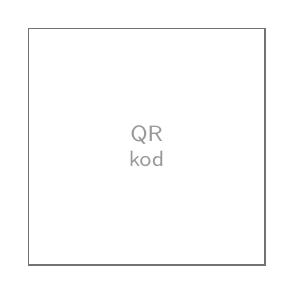
\begin{tikzpicture}
\draw[black!55,line width=0.6pt] (0,0) rectangle (30mm,30mm);
\node[black!40,font=\sffamily\fontsize{8}{9}\selectfont,align=center] at (15mm,15mm) {QR\\kod};
\end{tikzpicture}\\[1.5mm]
{\sffamily\fontsize{9}{11}\selectfont\color{black!70} #1}%
}

% ---- Answer-table styling: accent-colored grid, like the reference "Number | Answer" table ----
\arrayrulecolor{accent}
\setlength{\arrayrulewidth}{0.7pt}
\renewcommand{\arraystretch}{1.35}
\newcommand{\anstitle}[1]{{\sffamily\bfseries\color{accent}\fontsize{11}{13}\selectfont #1}\\[1.3mm]}

\begin{document}

% ================= PAGE 1: Set 1 | Set 2 =================
\topicheader{4}{So'z masalalarini tarjima qilish}
\pagefooter{22}
\colrule{32}{238}
\mbox{}%

\begin{textblock*}{\COLW}(\LCOL,32mm)
{\fontsize{11}{14}\selectfont
\setkicker{1-to'plam}{Faqat tarjima qiling -- javobni hisoblamang.}

\noindent\pnum{1} Bir son $x$ va 9 ning yig'indisi.\\[16mm]
\noindent\pnum{2} Bir son $n$ dan 7 kam.\\[16mm]
\noindent\pnum{3} Bir son $y$ 12 ga kamaytirilgan.\\[16mm]
\noindent\pnum{4} Bir son $x$ ning ikki bravari, 5 ga oshirilgan.\\[16mm]
\noindent\pnum{5} Bir son $n$ va 4 ning ko'paytmasi, 3 ga kamaytirilgan.\\[16mm]
\noindent\pnum{6} Bir son $x$ ning uch bravaridan 5 ko'p.\\[16mm]
\noindent\pnum{7} Bir son $n$ kamida 10.\\[16mm]
\noindent\pnum{8} Bir son $x$, 6 ga kamaytirilganda, 20 dan oshmaydi.
}
\end{textblock*}

\begin{textblock*}{\COLW}(\RCOL,32mm)
{\fontsize{11}{14}\selectfont
\setkicker{2-to'plam}{Tarjima qiling va yeching (bir qadamli).}

\noindent\pnum{1} Bir son $n$ dan 7 kami 15 ga teng. $n$ ni toping.\\[22mm]
\noindent\pnum{2} Bir son $x$ 9 ga oshirilganda 23 bo'ladi. $x$ ni toping.\\[22mm]
\noindent\pnum{3} Bir son $y$ ning ikki bravari 36 ga teng. $y$ ni toping.\\[22mm]
\noindent\pnum{4} Bir son 8 ga kamaytirilganda 15 bo'ladi. Sonni toping.\\[22mm]
\noindent\pnum{5} Bir son $m$ dan 15 kami 7 ga teng. $m$ ni toping.\\[22mm]
\noindent\pnum{6} Bir son $k$ ning 4 ga bo'linmasi 9 ga teng. $k$ ni toping.
}
\end{textblock*}

\clearpage

% ================= PAGE 2: Set 3 | Set 4 =================
\topicheader{4}{So'z masalalarini tarjima qilish}
\pagefooter{23}
\colrule{32}{238}
\mbox{}%

\begin{textblock*}{\COLW}(\LCOL,32mm)
{\fontsize{11}{14}\selectfont
\setkicker{3-to'plam}{Tarjima qiling va yeching (ikki qadamli).}

\noindent\pnum{1} Bir son $x$ ning ikki bravaridan 5 ko'pi 17 ga teng. $x$ ni toping.\\[24mm]
\noindent\pnum{2} Bir son $n$ ning uch bravaridan 8 kami 19 ga teng. $n$ ni toping.\\[24mm]
\noindent\pnum{3} Bir son $y$ va 4 ning yig'indisining ikki bravari 26 ga teng. $y$ ni toping.\\[24mm]
\noindent\pnum{4} Bir son $k$ ning yarmidan 7 kami 3 ga teng. $k$ ni toping.\\[24mm]
\noindent\pnum{5} Bir son $m$ ning to'rt bravaridan 3 kami, shu sonning ikki bravaridan 9 ko'piga teng. $m$ ni toping.\\[24mm]
\noindent\pnum{6} Bir son $x$, 6 ga kamaytirilib, ikki barobar oshirilsa, 28 bo'ladi. $x$ ni toping.
}
\end{textblock*}

\begin{textblock*}{\COLW}(\RCOL,32mm)
{\fontsize{11}{14}\selectfont
\setkicker{4-to'plam}{To'liq so'z masalalari (modellashtirish).}

\noindent\pnum{1} To'rtburchakning uzunligi eni ning uch bravaridan 2 ko'p. Perimetri 44. Enini toping.\\[26mm]
\noindent\pnum{2} Ikki ketma-ket butun sonning yig'indisi 45. Kichik sonni toping.\\[26mm]
\noindent\pnum{3} Mariya ukasining yoshidan ikki barobar katta va яна 4 yosh katta. Yoshlari yig'indisi 31. Ukasining yoshini toping.\\[26mm]
\noindent\pnum{4} Ko'ylak qalpoqdan ikki barobar qimmat va yana \$8 qimmat. Ikkalasi birgalikda \$38. Qalpoqning narxini toping.\\[26mm]
\noindent\pnum{5} Bir son o'zining 20\%-iga oshirilganda 72 bo'ladi. Dastlabki sonni toping.
}
\end{textblock*}

\clearpage

% ================= PAGE 3: Set 5 | Set 6 (spot the error) =================
\topicheader{4}{So'z masalalarini tarjima qilish}
\pagefooter{24}
\colrule{32}{238}
\mbox{}%

\begin{textblock*}{\COLW}(\LCOL,32mm)
{\fontsize{11}{14}\selectfont
\setkicker{5-to'plam}{Tengsizlikni tarjima qiling va yeching.}

\noindent\pnum{1} Bir son 5 ga kamaytirilganda kamida 10 bo'ladi. Sonning mumkin bo'lgan qiymatlarini toping.\\[24mm]
\noindent\pnum{2} Bir sonning uch bravari 21 dan oshmaydi. Mumkin bo'lgan qiymatlarni toping.\\[24mm]
\noindent\pnum{3} Bir sondan 5 ko'pi 12 dan kichik. Mumkin bo'lgan qiymatlarni toping.\\[24mm]
\noindent\pnum{4} Bir son ning ikki bravaridan 4 kami kamida 10. Mumkin bo'lgan qiymatlarni toping.\\[24mm]
\noindent\pnum{5} Faqat tarjima qiling: bir son $x$ 8 dan katta.
}
\end{textblock*}

\begin{textblock*}{\COLW}(\RCOL,32mm)
{\fontsize{10.5}{13.5}\selectfont
\setkicker{6-to'plam}{Xatoni toping -- "kam" so'zidagi tartib almashtirish xatosi.}

\noindent\pnum{1} Tarjima qiling: ``bir son $x$ dan 9 kam.'' -- \textit{berilgan: $9-x$.}\\[1mm]
\hspace*{7mm}Xato va to'g'ri javob: \makebox[52mm]{\dotfill}\\[8mm]

\noindent\pnum{2} ``Bir son $n$ dan 15 kami 20 ga teng. $n$ ni toping.'' -- \textit{berilgan: $15-n=20$.}\\[1mm]
\hspace*{7mm}Xato va to'g'ri javob: \makebox[52mm]{\dotfill}\\[8mm]

\noindent\pnum{3} Tarjima qiling: ``bir son $y$ dan 6 ayirilgan.'' -- \textit{berilgan: $6-y$.}\\[1mm]
\hspace*{7mm}Xato va to'g'ri javob: \makebox[52mm]{\dotfill}\\[8mm]

\noindent\pnum{4} Tarjima qiling: ``bir son $x$ 10 dan kichik.'' -- \textit{berilgan: $10-x$.}\\[1mm]
\hspace*{7mm}Xato va to'g'ri javob: \makebox[52mm]{\dotfill}\\[8mm]

\noindent\pnum{5} ``Bir son va 3 ning ayirmasining ikki bravari 10 ga teng. Sonni toping.'' -- \textit{berilgan: $2n-3=10$.}\\[1mm]
\hspace*{7mm}Xato va to'g'ri javob: \makebox[52mm]{\dotfill}
}
\end{textblock*}

\clearpage

% ================= PAGE 4: Set 7 (bonus) -- own page =================
\topicheader{4}{So'z masalalarini tarjima qilish}
\pagefooter{25}
\colrule{32}{238}
\mbox{}%

\begin{textblock*}{\COLW}(\LCOL,32mm)
{\fontsize{11}{14}\selectfont
\setkicker{7-to'plam}{Bonus / qiyin -- ko'p qadamli, vaqtni nazorat qiling.}

\noindent\pnum{1} Uchta ketma-ket juft butun sonning yig'indisi 90. Eng \textbf{katta} sonni toping.\\[32mm]
\noindent\pnum{2} Arqon ikki bo'lakka kesilgan. Bir bo'lagi ikkinchisining ikki bravaridan 5 metr uzun. Umumiy uzunligi 35 metr. Eng \textbf{qisqa} bo'lakning uzunligini toping.\\[32mm]
\noindent\pnum{3} Jonning puli Mariyaning pulidan ikki barobar ko'p va yana \$15 ko'p. Birgalikda \$120. \textbf{Jon}ning pulini toping.\\[32mm]
\noindent\pnum{4} Bir son o'zining 30\%-iga oshirilib, so'ng 5 ga kamaytirilsa, 47 bo'ladi. Dastlabki sonni toping.\\[32mm]
\noindent\pnum{5} Bir son va 7 ning yig'indisining ikki bravari, shu sonning besh bravaridan 10 kamiga teng. Sonni toping.
}
\end{textblock*}

\clearpage

% ================= PAGE 5: Javoblar -- full-page answer table, own page always =================
\topicheader{4}{So'z masalalarini tarjima qilish}
\pagefooter{26}
\mbox{}%

\begin{textblock*}{194mm}(16mm,30mm)
{\bfseries\itshape\color{accent}\fontsize{19}{21}\selectfont\centering Javoblar\par}
\end{textblock*}

\begin{textblock*}{194mm}(16mm,44mm)
{\fontsize{10}{12.5}\selectfont
\centering
\renewcommand{\arraystretch}{1.3}
\begin{tabular}{|>{\centering\arraybackslash}p{26mm}|>{\centering\arraybackslash}p{10mm}|>{\centering\arraybackslash}p{28mm}|>{\centering\arraybackslash}p{10mm}|>{\centering\arraybackslash}p{28mm}|}
\hline
\rowcolor{badge!55}\textbf{To'plam} & \textbf{\#} & \textbf{Javob} & \textbf{\#} & \textbf{Javob}\\
\hline
\multirow{4}{26mm}{\centering 1-to'plam} & 1 & $x+9$ & 2 & $n-7$\\\cline{2-5}
 & 3 & $y-12$ & 4 & $2x+5$\\\cline{2-5}
 & 5 & $4n-3$ & 6 & $3x+5$\\\cline{2-5}
 & 7 & $n\geq10$ & 8 & $x-6\leq20$\\\hline
\multirow{3}{26mm}{\centering 2-to'plam} & 1 & $n=22$ & 2 & $x=14$\\\cline{2-5}
 & 3 & $y=18$ & 4 & $x=23$\\\cline{2-5}
 & 5 & $m=22$ & 6 & $k=36$\\\hline
\multirow{3}{26mm}{\centering 3-to'plam} & 1 & $x=6$ & 2 & $n=9$\\\cline{2-5}
 & 3 & $y=9$ & 4 & $k=20$\\\cline{2-5}
 & 5 & $m=6$ & 6 & $x=20$\\\hline
\multirow{5}{26mm}{\centering 4-to'plam} & \multicolumn{4}{p{76mm}|}{1.\ eni $=5$ (uzunligi $=17$)}\\\cline{2-5}
 & \multicolumn{4}{p{76mm}|}{2.\ kichik son $=22$}\\\cline{2-5}
 & \multicolumn{4}{p{76mm}|}{3.\ ukaning yoshi $=9$}\\\cline{2-5}
 & \multicolumn{4}{p{76mm}|}{4.\ qalpoq narxi $=\$10$}\\\cline{2-5}
 & \multicolumn{4}{p{76mm}|}{5.\ dastlabki son $=60$}\\\hline
\multirow{3}{26mm}{\centering 5-to'plam} & 1 & $x\geq15$ & 2 & $x\leq7$\\\cline{2-5}
 & 3 & $x<7$ & 4 & $x\geq7$\\\cline{2-5}
 & 5 & $x>8$ & -- & --\\\hline
\multirow{5}{26mm}{\centering 6-to'plam} & \multicolumn{4}{p{76mm}|}{1.\ Xato -- tartib teskari bo'lishi kerak edi. To'g'ri: $x-9$.}\\\cline{2-5}
 & \multicolumn{4}{p{76mm}|}{2.\ Xato -- xuddi shu teskari tartib. To'g'ri: $n-15=20$, demak $n=35$.}\\\cline{2-5}
 & \multicolumn{4}{p{76mm}|}{3.\ Xato -- ``ayirilgan'' ham tartibni teskari qiladi. To'g'ri: $y-6$.}\\\cline{2-5}
 & \multicolumn{4}{p{76mm}|}{4.\ Xato -- bu solishtirish, ayirish emas. To'g'ri: $x<10$.}\\\cline{2-5}
 & \multicolumn{4}{p{76mm}|}{5.\ Xato -- ayirma qavsga olinishi kerak edi. To'g'ri: $2(n-3)=10$, demak $n=8$.}\\\hline
\multirow{3}{26mm}{\centering 7-to'plam} & 1 & $32$ & 2 & $10$ m\\\cline{2-5}
 & 3 & $\$85$ & 4 & $40$\\\cline{2-5}
 & 5 & $8$ & -- & --\\\hline
\end{tabular}
}
\end{textblock*}

\begin{textblock*}{194mm}(16mm,240mm)
\centering
{\sffamily\fontsize{9.5}{11.5}\selectfont\color{black!70} Video yechimlar va qo'shimcha testlar uchun quyidagi QR kodlarni skanerlang:}\\[4mm]
\begin{minipage}[t]{32mm}\centering\qrbox{YouTube}\end{minipage}%
\hspace{16mm}%
\begin{minipage}[t]{32mm}\centering\qrbox{Telegram}\end{minipage}
\end{textblock*}

\end{document}
